\let\negmedspace\undefined
\let\negthickspace\undefined
\documentclass[journal]{IEEEtran}
\usepackage[a5paper, margin=10mm, onecolumn]{geometry}
\setlength{\headheight}{1cm} 
\setlength{\headsep}{0mm}     
\usepackage{gvv-book}
\usepackage{gvv}
\usepackage{amsmath,amssymb,amsfonts,amsthm}
\usepackage{mathtools}
\usepackage{tikz}
\usepackage{gensymb}
\usepackage[breaklinks=true]{hyperref}

\begin{document}

\bibliographystyle{IEEEtran}
\vspace{3cm}

\title{2.9.22}
\author{AI25BTECH11006}
{\let\newpage\relax\maketitle}

\textbf{Question}: Let $\overrightarrow{a}$,
$\overrightarrow{b}$, and $\overrightarrow{c}$ be three vectors such that $|\overrightarrow{a}| = 1$, $|\overrightarrow{b}| = 2$, and $|\overrightarrow{c}| = 3$. If the
projection of $\overrightarrow{b}$ along $\overrightarrow{a}$ is equal to the projection of $\overrightarrow{c}$ along $\overrightarrow{a}$, and $\overrightarrow{b}$ and $\overrightarrow{c}$ are perpendicular to each other, then find $|3\overrightarrow{a} - 2\overrightarrow{b} + 2\overrightarrow{c}|$.

\textbf{Solution using Gram Matrix}:\\

Let us define the vector:
\begin{equation}
\vec{v} = 3\vec{a} - 2\vec{b} + 2\vec{c}
\end{equation}

\begin{equation}
\norm{\vec{v}}^2 = \vec{v}^T \vec{v}
\end{equation}

Let the Gram matrix be defined as:
\begin{equation}
G = \begin{bmatrix}
\vec{a}^T\vec{a} & \vec{a}^T\vec{b} & \vec{a}^T\vec{c} \\
\vec{b}^T\vec{a} & \vec{b}^T\vec{b} & \vec{b}^T\vec{c} \\
\vec{c}^T\vec{a} & \vec{c}^T\vec{b} & \vec{c}^T\vec{c}
\end{bmatrix}
\end{equation}

Let the coefficient vector be:
\begin{equation}
\vec{k} = \begin{bmatrix} 3 \\ -2 \\ 2 \end{bmatrix}
\end{equation}

Then,
\begin{equation}
\norm{\vec{v}}^2 = \vec{k}^T G \vec{k}
\end{equation}


\begin{equation}
\vec{a}^T\vec{a} = 1,\quad
\vec{b}^T\vec{b} = 4,\quad
\vec{c}^T\vec{c} = 9
\end{equation}

\begin{equation}
\vec{b}^T\vec{c} = 0,\quad
\vec{a}^T\vec{b} = d,\quad
\vec{a}^T\vec{c} = d
\end{equation}

\begin{equation}
\frac{\vec{b}^T \vec{a}}{\norm{\vec{a}}} = \frac{\vec{c}^T \vec{a}}{\norm{\vec{a}}}
\quad \Rightarrow \quad
\vec{b}^T\vec{a} = \vec{c}^T\vec{a}
\end{equation}

Thus, we can set $\vec{a}^T\vec{b} = \vec{a}^T\vec{c} = d$.

---


\begin{equation}
G = \begin{bmatrix}
1 & d & d \\
d & 4 & 0 \\
d & 0 & 9
\end{bmatrix}
\end{equation}


Computing $\norm{\vec{v}}^2$:

\begin{equation}
\norm{\vec{v}}^2 = 
\begin{bmatrix} 3 & -2 & 2 \end{bmatrix}
\begin{bmatrix}
1 & d & d \\
d & 4 & 0 \\
d & 0 & 9
\end{bmatrix}
\begin{bmatrix} 3 \\ -2 \\ 2 \end{bmatrix}
\end{equation}

Multiply step-by-step:

\begin{equation}
= 3(3 \times 1 + (-2)\times d + 2\times d) + (-2)(3\times d + (-2)\times 4 + 2\times 0) + 2(3\times d + (-2)\times 0 + 2\times 9)
\end{equation}

Simplifying:

\begin{equation}
= 3(3 + (-2d) + 2d) + (-2)(3d - 8) + 2(3d + 18)
\end{equation}

\begin{equation}
= 3(3) + (-2)(3d - 8) + 2(3d + 18)
\end{equation}

\begin{equation}
= 9 + (-6d + 16) + (6d + 36)
\end{equation}

\begin{equation}
= 9 + 16 + 36
\end{equation}

\begin{equation}
= 61
\end{equation}

Thus,

\begin{equation}
\norm{\vec{v}} = \sqrt{61}
\end{equation}


\begin{equation}
\boxed{\norm{3\vec{a} - 2\vec{b} + 2\vec{c}} = \sqrt{61}}
\end{equation}


\begin{figure}[h!]
   \centering
   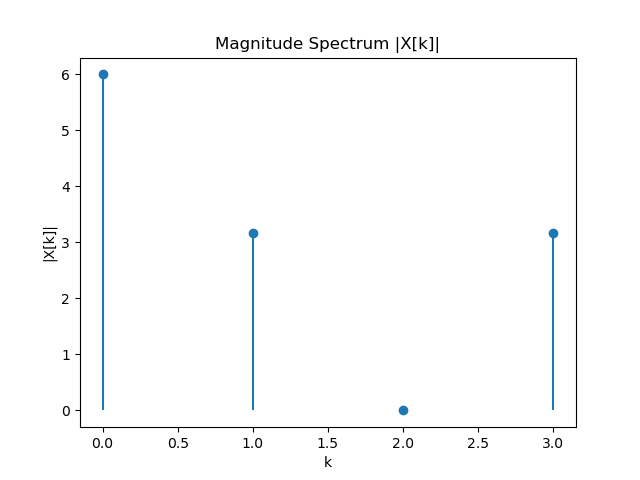
\includegraphics[width=1\linewidth]{fig1.png}
   \caption{}
   \label{stemplot}
\end{figure}



\end{document}  
